%
% File naacl2019.tex
%
%% Based on the style files for ACL 2018 and NAACL 2018, which were
%% Based on the style files for ACL-2015, with some improvements
%%  taken from the NAACL-2016 style
%% Based on the style files for ACL-2014, which were, in turn,
%% based on ACL-2013, ACL-2012, ACL-2011, ACL-2010, ACL-IJCNLP-2009,
%% EACL-2009, IJCNLP-2008...
%% Based on the style files for EACL 2006 by 
%%e.agirre@ehu.es or Sergi.Balari@uab.es
%% and that of ACL 08 by Joakim Nivre and Noah Smith

\documentclass[11pt,a4paper]{article}
\usepackage[hyperref]{naaclhlt2019}
\usepackage{times}
\usepackage{graphicx}
\usepackage{booktabs}
\usepackage[ruled,vlined]{algorithm2e}
\usepackage{latexsym}
\usepackage{amsmath}
\usepackage{amssymb}
\usepackage{bm}

\newcommand{\rdep}[1]{\ $\xrightarrow{\text{\tiny #1}}$\ }


\newcommand{\ahcomment}[1]{\textcolor{blue}{[#1 -AH]}}

\usepackage{url}

%\aclfinalcopy % Uncomment this line for the final submission
%\def\aclpaperid{***} %  Enter the acl Paper ID here

%\setlength\titlebox{5cm}
% You can expand the titlebox if you need extra space
% to show all the authors. Please do not make the titlebox
% smaller than 5cm (the original size); we will check this
% in the camera-ready version and ask you to change it back.

%\hypersetup{draft} % THIS IS NEEDED TO GET IT TO COMPILE. Does not like the tables. AH 11/27

\newcommand\BibTeX{B{\sc ib}\TeX}

\DeclareMathOperator*{\argmaxA}{arg\,max} % Jan Hlavacek

% Extractive sentence compression under lexical and length constraints
\title{Additive Compression with Lexical and Length Constraints}

\author{First Author \\
  Affiliation / Address line 1 \\
  Affiliation / Address line 2 \\
  Affiliation / Address line 3 \\
  {\tt email@domain} \\\And
  Second Author \\
  Affiliation / Address line 1 \\
  Affiliation / Address line 2 \\
  Affiliation / Address line 3 \\
  {\tt email@domain} \\}

\date{}

\begin{document}
\maketitle

\begin{abstract}
Extractive sentence compression seeks to reduce the length of a sentence, while retaining the most ``important'' information from the source. But query-focused applications such as document search engines or exploratory search interfaces place additional length, lexical and latency constraints on compression systems. This study introduces a new transition-based technique, developed for such settings. Our method constructs compressions in linear time by growing a forest in a dependency parse, achieving a 100X speed up over traditional ILP-based methods. Our technique also better reconstructs known-good shortenings under constraints.
\end{abstract}

\section{Introduction}\label{s:intro}

Traditional study of extractive sentence compression seeks to create short, readable compressions which retain the most ``important'' information from source sentences. But query-focused and user-facing applications impose additional requirements on the output of a compression system. Compressions must be short enough to be shown in a user interface and often must contain a user's query term, which defines the ``important'' information in the sentence. Query-focused applications applications also require low latency to support interactive browsing. An example application is shown in Figure \ref{f:qf}.

\begin{figure}[htb!]
%\fbox{
%\begin{minipage}{7.6 cm}
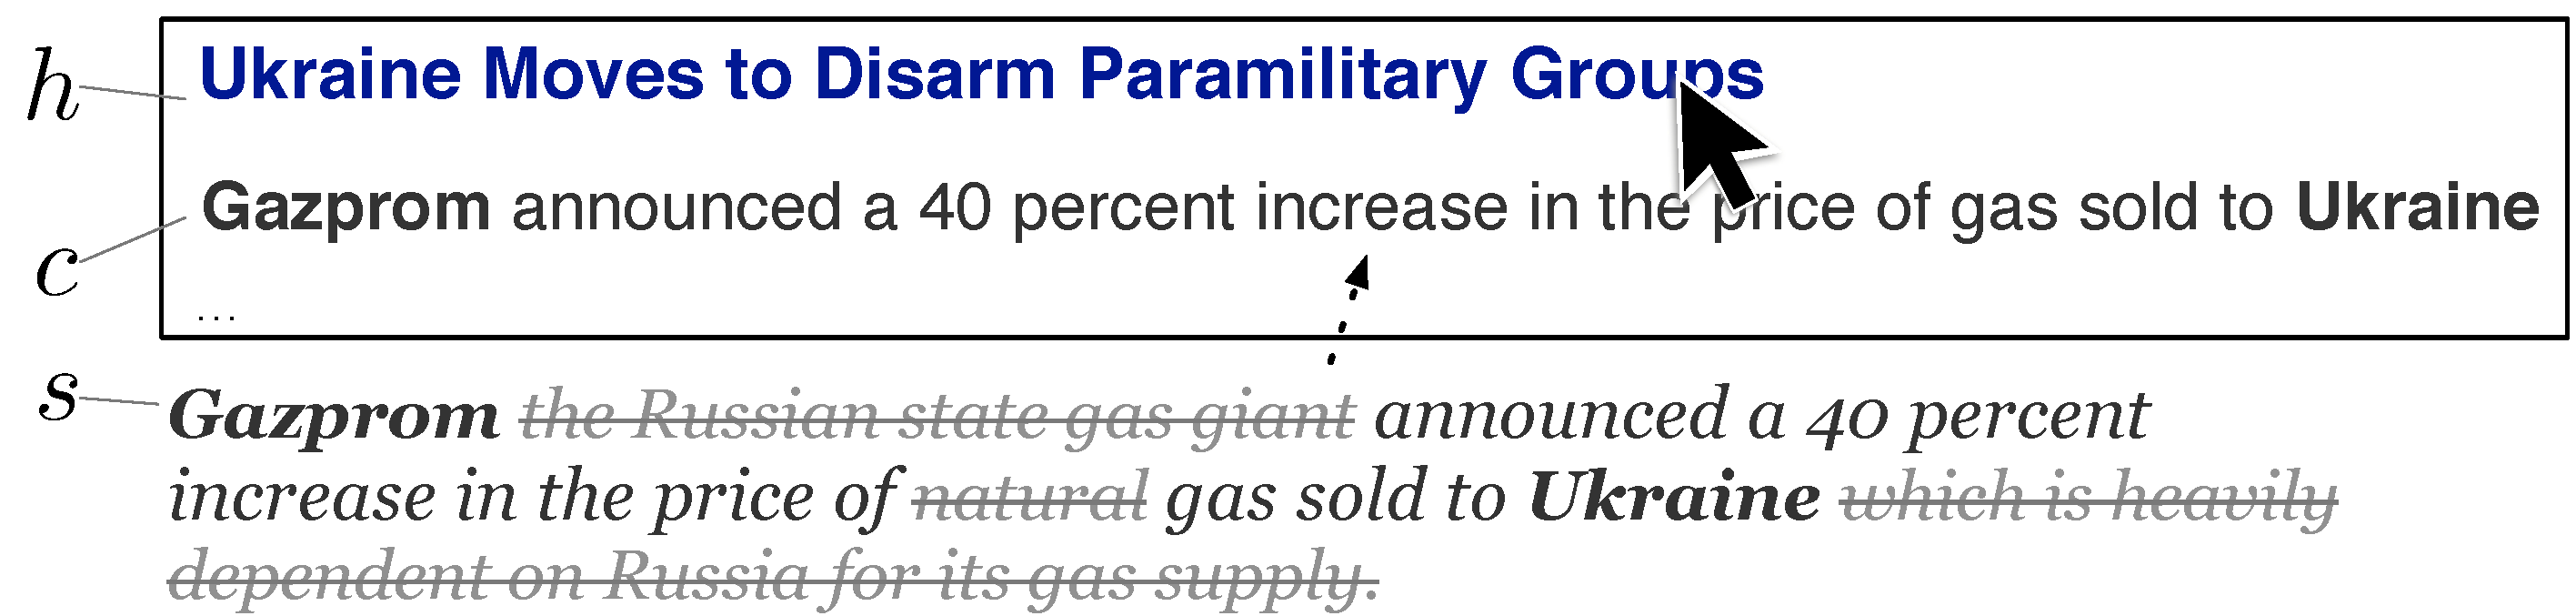
\includegraphics[width=8.5cm]{qf.pdf}
\caption{A search interface (boxed, top) returns a headline $h$ above a constrained compression $c$, shortened from a sentence $s$ in a query-relevant document (italics, bottom). The constrained compression must contain the users' query terms (bold), and must not exceed 75 characters in length.}
\label{f:qf}
%\end{minipage}
%}
\end{figure}

This study examines the English-language compression problem with such length and lexical requirements. In constrained compression, source sentences $S$ are shortened to compressions $C$ which (1) include query words $Q$ and (2) are shorter than or equal in length to a maximum character length, $b \in \mathbb{Z}^{+}$. Formally, the task is to construct a function $(S,Q,b) \rightarrow c$, such that $c$ respects $Q$ and $b$.

Older compression methods  \cite{clarke2008global,filippova2013overcoming} based on integer linear programming can trivially accommodate such restrictions, but rely on slow third-party solvers to optimize an NP-hard integer linear programming objective\label{s:relatedwork}. Newer sequence to sequence methods \cite{filippova2015sentence} do not allow practitioners to specify length or lexical constraints, and require access to specialized graphics processing hardware (GPU) to achieve low latency which is a barrier for practitioners in fields like social science and journalism. These deficits make existing compression techniques unsuitable for search engines \cite{hearst2009search}, concept map browsers \cite{falke2017graphdocexplore} and new forms of exploratory textual interfaces \cite{marchionini2006exploratory}, where length, lexical and latency constraints are paramount. 

\begin{table*}[htb!]
\begin{tabular}{lccc}
\textbf{Approach} & \textbf{Worst-case complexity} & \textbf{Constrained}  \\ \hline
Sequence to sequence taggers \cite{filippova2015sentence}   & linear              & no         \\   
\textbf{Additive compression (this work)}  & \textbf{linear}     &      \textbf{yes}   \\
ILP    \cite{filippova2013overcoming,Wang2017CanSH}       &   exponential    & yes      \\
\end{tabular}
\caption{Supervised ILP compression methods \cite{clarke2008global,filippova2013overcoming,Wang2017CanSH} can easily accommodate length and lexical restrictions. But these methods must solve a known NP-hard problem with worst-case exponential runtime. LSTM taggers \cite{filippova2015sentence} achieve comparable results with linear runtime, but cannot accommodate length or lexical requirements. This work introduces a supervised additive approach (\S\ref{s:system}) which shortens sentences under constraints in linear time.} 
\label{t:algos}
\end{table*}

We thus present a new method for constrained compression which grows a forest in a dependency parse in linear time. We compare this \textit{additive compression} method to supervised, integer linear programming (ILP) systems, which also accommodate length and lexical restrictions. Our method has lower theoretical and empirical computational costs, while better reconstructing known-good shortenings. 

\section{Related work}\label{s:relatedwork}

Extractive compression shortens a sentence by removing tokens \cite{Knight2000StatisticsBasedS,clarke2008global,filippova2015sentence,Wang2017CanSH}, typically for extractive summarization \cite{Knight2000StatisticsBasedS,almeida2013fast,P16-1188}.\footnote{Some methods shorten sentences via generation instead of deletion \cite{rush2015neural,mallinson18}. Our interest in the extractive setting follows from a motivation to create interpretable,  trustworthy, and practical search systems \cite{Chuang2012InterpretationAT}: users might not trust abstractive summaries \cite{Zhang:2018:MSG:3290265.3274465}, particularly in cases with semantic error.} To our knowledge, this work is the first to consider extractive compression under length and lexical constraints.\footnote{\citet{Li2013DocumentSV} solicit annotations for ``guided'' compression, but do not examine the compression problem under lexical and length constraints.}

Our interest in constrained compression is motivated by search user interfaces \cite{hearst2009search}, which require query-biased snippets for search engine results pages \cite{tombros1998advantages}.\footnote{Version 7.5 of Apache Lucene, the leading open source search engine, does not perform sentence compression in generating snippets. \url{https://lucene.apache.org/core/7_5_0/highlighter/index.html}} New search interfaces such as concept map browsers could also make use of constrained compressions \cite{marchionini2006exploratory,emnlp2017conceptmaps}. Because such user-facing systems require low-latency \cite{Nielsen,heerschei,Liu2014TheEO}, we prioritized computational efficiency in designing a solution to the constrained task. We also avoided neural approaches which achieve low latency with expensive GPUs.

We compare our approach to ILP compression techniques \cite{clarke2008global,filippova2008dependency,filippova2013overcoming,Wang2017CanSH}, which can easily specify that optimal solutions need to be shorter than some character budget, and need to include query terms. However, the task of identifying the global optimum of such an integer programming objective is a well-known, NP-hard problem \cite{clarke2008global}, requiring worst-case exponential computation in the length of the input sequence. In practice, ILP methods use off-the-shelf solvers to identify the highest-scoring compression, from among all possible configurations of binary variables. 

At this time, sequence to sequence sentence compression \cite{filippova2015sentence} is unsuitable for query-focused applications because such methods cannot enforce lexical or length requirements. This limitation might be reexamined in future work, by modifying or adapting new constrained generation techniques \cite{N18-1119,aaimh}.

\section{Additive compression}\label{s:system}

In this work, we present a new transition-based method for shortening sentences under lexical and length constraints, inspired by similar approaches in transition-based parsing \cite{nivre2003}. We describe our technique as additive compression, because it constructs a shortening by \textit{growing} a forest in the dependency parse of a sentence. This approach differs from some prior work which
compresses sentences by \textit{pruning} subtrees \cite{Jing2000SentenceRF,Knight2000StatisticsBasedS,berg2011jointly,almeida2013fast,Filippova2015FastKS,filippova2015sentence}. 

The chief advantage of additive compression is that it can construct constrained compressions in linear rather than exponential time (\S\ref{s:costs}). Such gains translate to lower latency while achieving better performance in constrained compression than supervised ILPs (\S\ref{s:autoeval}).

\subsection{Additive procedure}\label{s:formal}

Our method builds a compression by maintaining a state
$(C_i,F_i)$ where $C_i \subseteq S$ is a set of compression tokens, $F_i  \subseteq S$ is a set of frontier tokens, and $i$ indexes a timestep during compression. Figure \ref{f:walkthru} shows a step-by-step example. 

During initialization, we set $C_0 \gets Q$ and $F_0 \gets S \setminus Q$. Then, at each timestep, we decide to either add or not add some vertex $v_i \in F$ to $C$. We discuss such decisions in detail in \S\ref{s:modeling}. At each timestep, we also remove $v_i$ from $F$. We continue adding vertexes to $C$ until either $F$ is empty or the linearized compression, $\ell(C)$, is longer than the length constraint.\footnote{We linearize tokens in their original sentence order, which is typical in English-language compression.} The appendix details the process with a formal algorithm.

We select $v$ from $F$ according to some policy $\pi$, denoted $v = \pi(F)$. In this work we use a rule-based policy: neighbors of $C$ are selected from $F$ before non-neighbors. If more than one neighboring (or non-neighboring) vertex is in $F$, we choose the leftmost vertex in the sentence from among possible choices.
 
\begin{figure}[h]
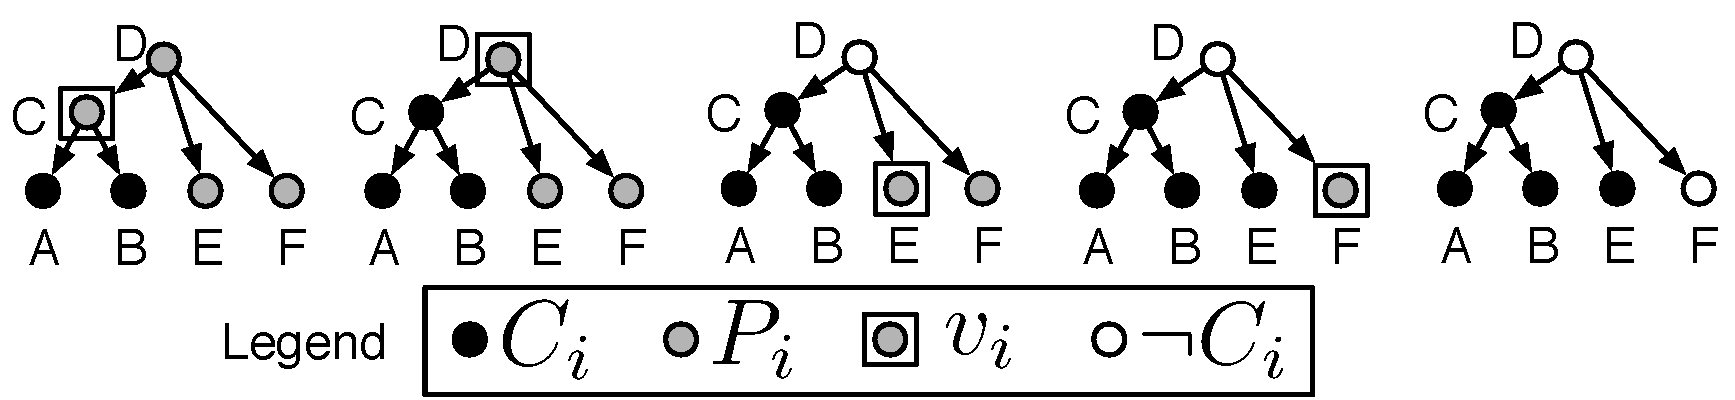
\includegraphics[width=8.2cm]{additive.pdf}
\caption{Additive compression in 5 timesteps, from left to right. Each $C_i$ is shown in black and each $F_i$ is shown in grey. The vertex $v= \pi(F)$ is shown as a square. The final compression is $\{1,2,3,5\}$. At initialization (far left), $C_0 \gets Q = \{1,2\}$ and $F_0 \gets S \setminus Q$.  }
\end{figure}\label{f:walkthru}


\subsection{Inclusion decisions}\label{s:modeling}

Additive compression decides to add or not add some vertex $v_i$ at each timestep $i$. We learn such decisions using a corpus of tuples $(S,Q,b,C_g)$, where $C_g$ is some known-good compression of $S$ respecting $Q$ and $b$ (\S\ref{s:intro}). Given $(S,Q,b,C_g)$ and $\pi$ we can construct a unique oracle compression path by initializing $C_0$ with $Q$, following $\pi$, and choosing to add $v_i$ to $C_i$ iff $v_i \in C_g$. 

We then use such oracle paths to train a model of oracle inclusion decisions, ${p(y_i  = 1 | v_i, C_i, F_i, S_i)}$. We discuss our model in (\S\ref{s:transition}). Our oracle procedure can reconstruct all compressions in a large, standard corpus \cite{filippova2013overcoming}. 

\section{Evaluation}\label{s:autoeval}

We compare additive compression to a supervised ILP baseline in terms of latency, readability and token-level F1 score. F1 is the standard automatic evaluation metric for the compression task, used to measure how well each compression method can reconstruct known-good shortenings. Our method achieves higher F1 scores, higher automatic readability scores and 100X lower latency (Table \ref{t:results}). We evaluate the significance of each difference with bootstrap sampling \cite{D12-1091}. All differences are significant {\small $(p < 10^{-2})$}. 

\subsection{Synthetic constrained compression experiment}

In order to evaluate different approaches to constrained compression, we require an evaluation dataset of sentences, constraints and known-good shortenings which respect the constraints. Formally, this means we need tuples $(S, Q, b, C_g)$, where $C_g$ respects $Q$ and $b$ (\S\ref{s:intro}).

To support large-scale automatic evaluation, we reinterpret a standard compression corpus \cite{filippova2013overcoming}
as a collection of input triples and constrained compressions.\footnote{See appendix for discussion of preprocessing.} For each $S$--$C_g$ pair in the dataset, we define $b$ as the character length of $C_g$. We then sample a query $Q$ from the tokens in $C_g$, based on the observed distribution of token counts \cite{Jansen2000RealLR}, and observed distribution of part-of-speech tags \cite{Barr2008TheLS} from real-world searches.\footnote{We reject samples in which the query length is longer than 6 tokens, which are poorly suited our setting. We manually map part-of-speech tags from \citet{Barr2008TheLS} to Penn tags, described in supporting code. We reject sampled part-of-speech tags which occur in fewer than 5\% of real queries.} Because we mimic real world behavior, search queries are often short (several tokens long), and often restricted to particular parts of speech (nouns and proper nouns). Sampled queries include ``police, Syracuse'', ``NHS'' and ``Hughes, manager, QPR.'' By sampling queries and defining budgets in this manner, we create a dataset of \ahcomment{X} tuples of the form $(S,Q,b,C)$.

\begin{table}[]
\begin{tabular}{lrrl}
\centering
Approach & F1 & SLOR &  Speed {\small (ms / $S$)}  \\ \hline
ILP &  {\small 0.854}   &  {\small 0.776 }  & {\small $\mu=$ .115} ({\small $ \sigma=.074$}) \\
Additive &  {\small \textbf{0.875}}  & {\small \textbf{0.800} }& {\small $\mu=$ 300} ({\small $ \sigma=X$}) \\
Rand.  &  {\small 0.690}  & { X }& {\small $\mu=$ 300} ({\small $ \sigma=X$}) \\
\end{tabular}
\caption{Test F1 scores, SLOR scores and average latency for three compression methods, for the constrained compression task. The difference between all metrics is statistically significant {\small $(p < 10^{-2})$}. Additive compression with random decisions (Rand.) achieves F1 = 0.690, which is the lower bound for this task.}
\label{t:results}
\end{table}

%Our experiment provides the oracle compression length to each compression system (via the parameter $b$). Automatic performance of compression systems is known to reflect their compression rate \cite{napoles2011evaluating}. We observe that both the ILP and the transition-based compressor achieve higher F1 in the constrained task than in the unconstrained setting.

\subsection{Implementation: transition-based compression}\label{s:transition}

We learn a model $p(y_i  = 1 | v_i, C_i, F_i, S_i)$ to perform compression. Instead of a neural approach \cite{D14-1082}, we implement feature-based, binary logistic regression which can run quickly without access to a GPU. This allows our method to be used in search applications in fields like social science and journalism, where expensive custom hardware is not available. The features in our model fall into two classes.

\textbf{Local features} describe the properties of the edge $(u,v)$ between $v \in F$ and $u \in C$. Such features are based on previous approaches to supervised non-neural sentence compression \cite{filippova2013overcoming,almeida2013fast,Filippova2015FastKS}, including structural features (e.g.~vertex depth in tree), lexical features, and semantic features (e.g.~NER tag). Our local features indicate if $u$ governs $v$ or vice versa. This allows our model to reason about the sorts of governors which should be included in a compression (e.g.~verbs) and the sorts of dependents which might not be added to $C$ (e.g.~modifiers). We describe the features in detail in our appendix and supporting code. If $v$ is disconnected from $C$, as in step 3 of Figure \ref{f:walkthru}, no local features are used.

\textbf{Global features} represent the relationship between $v$ and the overall compression $C$. Global features include information such as the position of $v$ in the sentence, relative to the right-most and left-most vertex in $C$. Such global features allow the feature-based model to reason about which sort of vertexes should be added to compressions in general. For instance, global features allow the model to learn if the oracle tends to include or not include gaps.

The appendix contains additional details regarding model tuning and implementation.

\subsection{Implementation: ILP-based compression}\label{s:ilp}

We compare our system to a state-of-the-art, ILP-based method, presented in \citet{filippova2013overcoming}. This approach represents each edge in a syntax tree with a vector of binary features, then learns weights for each feature using a structured perceptron trained on a corpus of $(S,C_g)$ pairs. Learned weights are used to compute a global compression objective, subject to structural constraints which ensure the output is a valid tree.

To our knowledge, a public implementation of this method does not exist. We reimplement from scratch using \citet{gurobi}, achieving a test-time, token-level F1 score of  0.690 on the unconstrained compression task, lower than the than the result reported by the original authors. There are some important differences between our reimplementation and the method reported in \citet{filippova2013overcoming}. We describe these differences in detail in the appendix.

\subsection{Importance and readability evaluation}\label{s:readabilityinformativeness}

Researchers often use human judgements of \textit{importance} and \textit{readability} to evaluate extractive sentence compression techniques \cite{Knight2000StatisticsBasedS,clarke2008global,filippova2015sentence}. In our constrained compression setting, $Q$ determines the ``important'' information from $S$. Thus, human importance evaluations are inappropriate.

We use the automated SLOR metric \cite{lau2015unsupervised} to check the readability of compressions. Prior work shows that this metric correlates with human readability judgements for the compression task \cite{kannConl}. SLOR normalizes the probability of a token sequence assigned from a language model, by adjusting for both the probability of the individual unigrams in the sentence and for the sentence length.\footnote{Longer sentences are always less probable than shorter sentences; rarer words make a sequence less probable.} Based on SLOR scores, our method might produce slightly more readable compressions (Table \ref{t:results}). The appendix details our implementation of SLOR. 

\subsection{Latency evaluation}\label{s:costs}

ILP-based approaches to sentence compression formalize the task as an integer linear programming optimization task, a well-known NP-hard problem  (\S\ref{s:relatedwork}), with exponential worst-case complexity.\footnote{The complexity is exponential in $|V|$ if the ILP selects tokens like \citet{clarke2008global}, and exponential in $|E|$ if the ILP selects edges like \citet{filippova2008dependency} or \citet{filippova2013overcoming}.} One advantage of our transition-based framework is that it can perform query-focused, budget-constrained compression that is linear in $|V|$, the token length of $S$. Compression is linear because we initialize the frontier $F$ with all $v_i \in V \setminus Q$, and then remove one vertex $v_i$ from $F$ at each timestep until $F$ is empty.

We test if the theoretical advantage of our system translates to a practical speedup by sampling 10,000 sentences with replacement from the test set, and performing compression with an ILP. We then repeat this experiment with our additive compression approach (Table \ref{t:results}). Our linear additive technique is \ahcomment{TODO} faster than existing methods. The appendix contains additional computational details.

\section{Conclusion and future work}

This work introduces a new additive method for extractive sentence compression, which is more computationally efficient than ILP-based methods and better reconstructs known-good sentence shortenings under constraints. 

%Finally, some shortened sentences will modify the meaning of a sentence. Identifying such cases is a special case of the unsolved textual entailment problem \cite{snli_bowman,Pavlick2016SoCalledNA,linzencompression}. In the future, we plan to apply entailment research to the compression task.  

% ack => Katie, Javier, NLP reading group! 

%\appendix

\begin{figure*}[htb!]
\centering
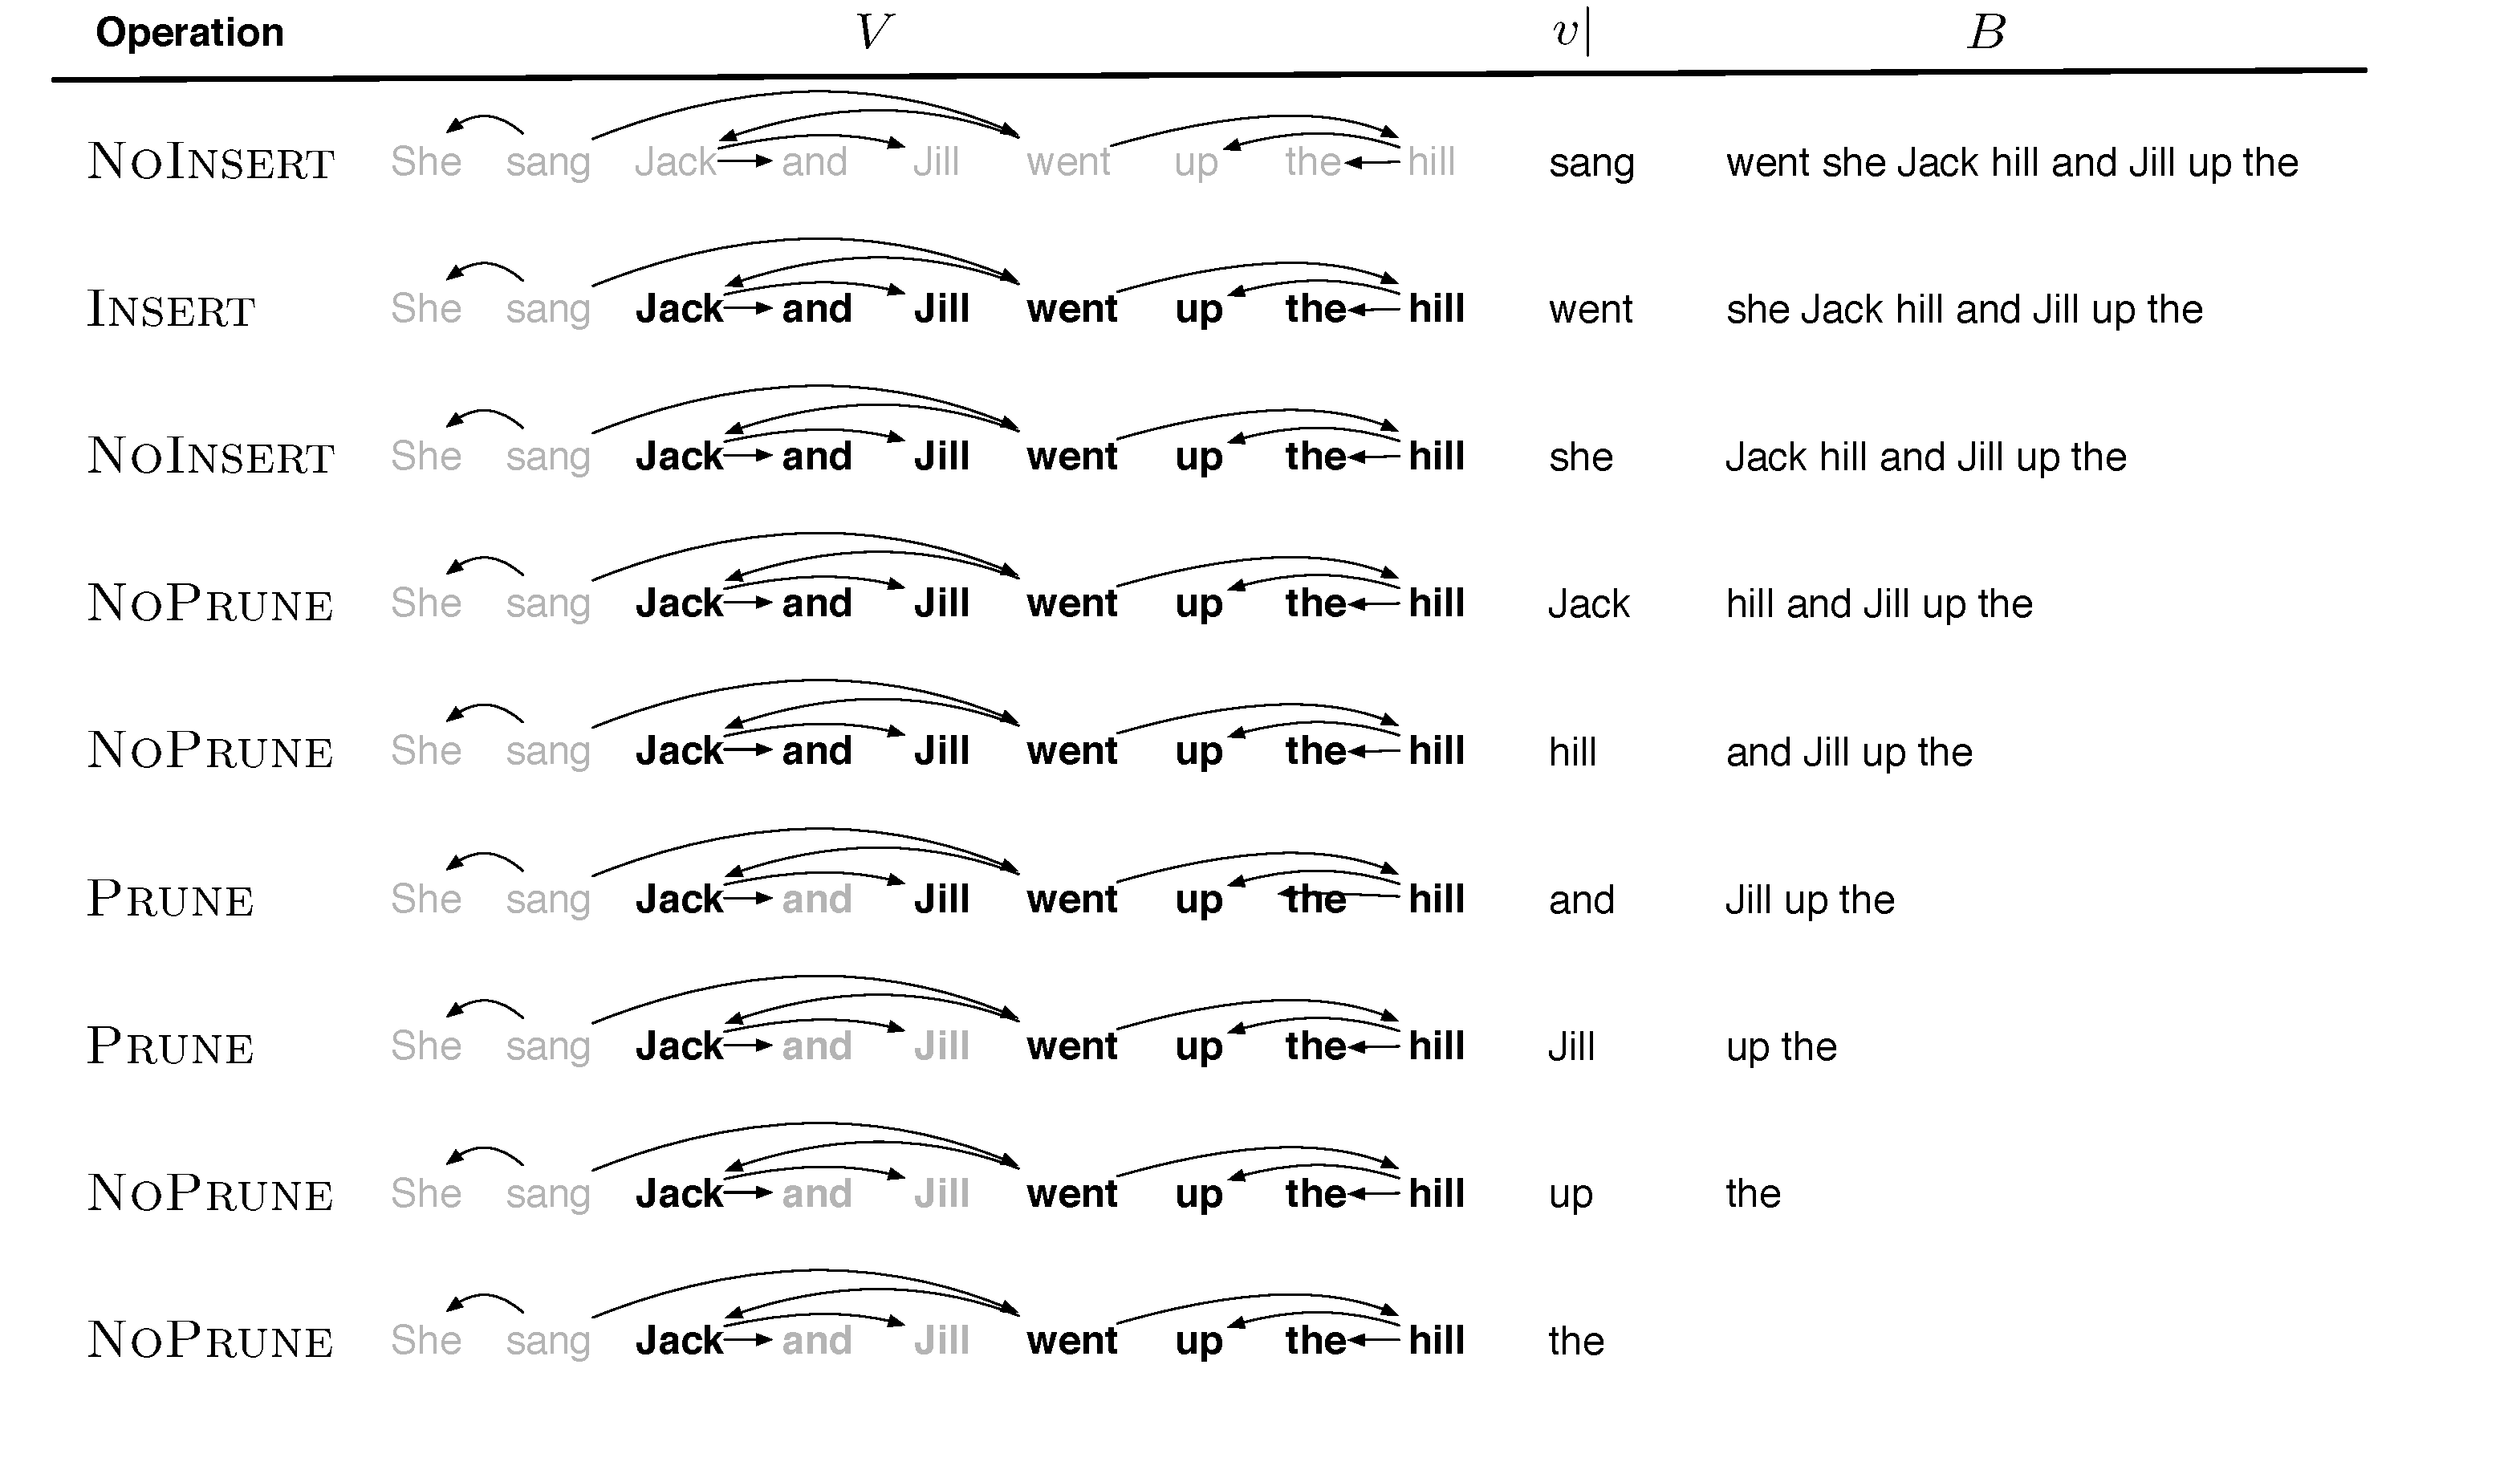
\includegraphics[width=.75\textwidth]{worked.pdf}
\caption{Nine operations of our transition-based compression return the compression: ``Jack went up the hill". At each timestep, the compression has state $(V_j, [v_j|B])$. In the diagram, the tokens in $V_j$ are shown in bold. The token $v_j$ is shown in the third column.}
\label{f:example}
\end{figure*}

\section{Appendix}


\subsection{Reimplementation of \citet{filippova2013overcoming}: additional details}

In this work, we reimplement the method of \citet{filippova2013overcoming}, who in turn implement a method partially described in \citet{filippova2008dependency}.  There are inevitable discrepancies between our implementation and the methods described in these two prior papers.  

Some discrepancies arise from differences in syntactic formalisms. To begin, prior work uses a tree transformation method which is no longer strictly compatible with UD. For instance, the tree transformation from prior work assumes PPs are headed by prepositions, which is not true in UD \cite{Schuster2016EnhancedEU}. We thus reimplement the tree transformation, using the enhanced dependencies representation from CoreNLP, which provides off-the-shelf augmented modifiers and augmented conjuncts that are very similar to the augmented edge labels from prior work. We exclude a syntactic constraint based on the \rdep{sc} relation, which is not included in UD.

Other possible discrepancies arise from differences in part-of-speech taggers. In particular, the aforementioned tree transform from prior work adds an edge between the root node and all verbs in a sentence, as a preprocessing step. This ensures that subclauses can be removed from parse trees, and then merged together to create a compression from different clauses of a sentence. However, we found that replicating this transform literally (i.e. only adding edges from the original root to all ``verbs'') made it impossible for the ILP to recreate some of the gold compressions in the dataset. (We suspect that this is because our part-of-speech tagger and the original part-of-speech tagger employed in \citet{filippova2013overcoming} sometimes return different part-of-speech tags). Our tree transform therefore adds an edge between the root node and \textit{all} tokens in a sentence. With this change, it is always possible for the ILP to output the gold compression.

We use \citet{gurobi} (v7) to solve the liner program. \citet{filippova2008dependency} report using LPsolve.\footnote{\url{http://
sourceforge.net/projects/lpsolve}}  We found that Gurobi sometimes segfaults nondeterminsitically during training. We implement checkpoints which save and restore the state of computation, allowing us to resume training when such errors occur.  We assess convergence by examining the validation F1 score on the constrained task after each pass through the training data. The F1 score increases for each of eight passes through the training data, and then decreases slightly (drops by $10^{-3}$ points). We terminate training at this point. 

Lastly, in Table 1 of their original paper, \citet{filippova2013overcoming} provide an overview of the syntactic, structural, semantic and lexical features in their model. We implement every feature explicitly described in their work, except where otherwise noted (e.g. syntactic feature not compatible with UD). However, additional features included in their model (but not explicity described in print) almost certainly affect performance. 

\subsection{Implementation of SLOR: additional details}

We use the SLOR function to measure the readability of the shortened sentences produced by each compression system. Following \cite{lau2015unsupervised}, we define the function as 

\begin{equation}
\text{SLOR}=\frac{\text{log}P_m(\xi) - \text{log}P_u(\xi)}{|\xi|}
\end{equation}

where $\xi$ is a sequence of words, $P_u(\xi)$ is the unigram probability of this sequence of words and $P_m(\xi)$ is the probability of the sequence, assigned by a language model.  $|\xi|$ is the length (in tokens) of the sentence.

We use a 3-gram language model trained on the \citet{filippova2013overcoming} corpus. We implement with KenLM \cite{Heafield-kenlm}.

\subsection{Subtree and compression brackets: additional details}\label{s:subtree}

Our markup input to our LSTM, $\bm{x}_j$, includes \textbf{subtree brackets} with a complex structure, used to represent the start and end of the tokens which will be pruned or inserted by an operation $o_j \in \{ \textsc{Prune},\textsc{Insert}\}$. The start and end tags are each formed by concatenating two symbols: (1) a symbol $o_j$ indicating the type of the operation proposal (i.e. prune or insert) and (2) a symbol $d$ indicating the dependency type governing $T(v)$, such as \texttt{dobj}. 

Additionally, the markup includes \textbf{compression brackets} which show the extent of the current compression (if the operation is \textsc{Prune}) or the extent of the compression which would result if the operation were to be accepted (if the operation is \textsc{Insert}). Concretely, these brackets show the extent of \textsc{Max}($V_{j+1}, V_{j}$) within $s$ where, \textsc{Max} selects the largest set by cardinality and where $V_{j+1}$ is all tokens which would be in $V$ at step $j+1$, if the system were to execute operation $o$ at timestep $j$. If $o_j=\textsc{Prune}$ then $V_{j+1}$ will be smaller than $V_j$ and the bracket symbols will show the extent of the current $V_j$. If $o_j=\textsc{Insert}$, then $V_{j+1}$ will be larger than $V_j$ and the compression brackets will show the extent of the compression which would result if the tokens were to be inserted. 

\subsection{Neural net training: additional details}

We note several additional details about our neural network training procedure, including hyperparameter settings.


\begin{table}[htb!]
\begin{tabular}{@{}ll@{}}
\toprule
Batch size         & 135                      \\ 
Hidden size        & 907                        \\
Embeddings dim.    & 300                      \\
Total fully-connected layers & 2                        \\
Fully-connected layers, hidden sizes & $(92, 2)$ \\
Fully-connected layers, dropout & $(0.309, 0.408)$ \\
Fully-connected layers, activations        & Relu, Linear             \\
Learning rate      & $4.593 * 10^{-4}$   \\
Weight decay       & $2.421 * 10^{-8}$   \\ \bottomrule
\end{tabular}
\caption{The hyperparameters for our model. The learning rate and weight decay parameter each clearly affect validation accuracy. The importance of other parameters is less clear. } 
\end{table}

\begin{itemize}
\item{We train on 8 million tuples. The cardinality of the training set was bounded by available hardware resources, not by the total number of oracle tuples which can be generated with the \citet{filippova2013overcoming} dataset.}
\item{We weight each training instance $(\bm{x_j}, y_j)$ using the default class weighting scheme in Scikit-learn \cite{Pedregosa:2011:SML:1953048.2078195}. The formula for assigning weights is $\frac{T_o}{2 * T_{o,j}}$. $T_o$ is the total number of training examples of accepted and rejected instances of the operation proposal $o$ (e.g. $T_o$ = total number of \textsc{Prune} examples + total number of \textsc{NoPrune} examples). $T_{o,j}$ is the total number of training operations labeled $y_j$ for operations of proposal type $o$ (e.g. $T_{o,j}$ = the total \textsc{NoPrune} operations, if $y_j=0$ and $o$ = \textsc{Prune}). The 2 in the numerator denotes the total number of classes. Alternative weighting methods are left for future work.}
\item{We experimented with ELMo vectors \cite{Peters:2018}, but found that we were able to achieve similar validation accuracies with much smaller embeddings. It is possible that ELMo-like vectors could be used to increase performance in the future.}
\end{itemize}

\bibliography{abe}
\bibliographystyle{acl_natbib}

\bibliography{abe}
\bibliographystyle{acl_natbib}

\end{document}

%\ahcomment{Sort of hard to tell what formalism F and A use. I thnk it is stanford, but they don't come out and say it.They cite Nivre's book which references the malt parser which seems to use stanford deps. but I don't see mention of the ``in" relation referenced in F and A paper in a guide to stanford deps. Writing around it.}

% other ideas... 
 
%\section{Computational experiments part 2: investigating properties of q,s,r compression}

%\ahcomment{include?}

%\ahcomment{only outline / notes here}

%\begin{enumerate}
%\item{q = a list of 1 to 3 NER}
%\item{r = random}
%\item{What is the size of the minimum compression?}
%\item{Reachability by budget by position of q in syntax tree. (If q is more than one entity then how the entities are dispersed across the tree probably matters a bunch too).}%
%\item{Hang on. reachability == min compression, eh? if min compression $>$ b, it is clearly bad.}
%\item{Avoid computational waste w/ grammar.  Examine: ops you never have to worry about if you prune a branch v. dependency type deletion endorsement rate. Some ops get rid of lots of tokens w/ very high probability of deletion endorsements: e.g. parataxis (a great op!). By contrast: pruning a noun subj destroys acceptability and usually does not delete many tokens. Not worth the risk!}
%\item{What is the empirical number of ops (i.e. decisions you have to make about pruning) if you greedily drop branches but never drop if the single op probability is less than $p$? My guess is you can make this problem way, way, simpler than implied by exponential formulation. Is it really quadratic?}
%\item{Distribution of number of ops used for different q and r: when choosing ops at random? when choosing greedily? When pruning $\propto$ p(endorsement)?}
%\item{Other stuff: min compression, reachability, operations saved w/ big prunes? position of query in the tree?}
%\end{enumerate}
